\section{
برنامه مدیریت هزینه‌های پروژه
}

\begin{center}
  \begin{figure} [h!]
    { 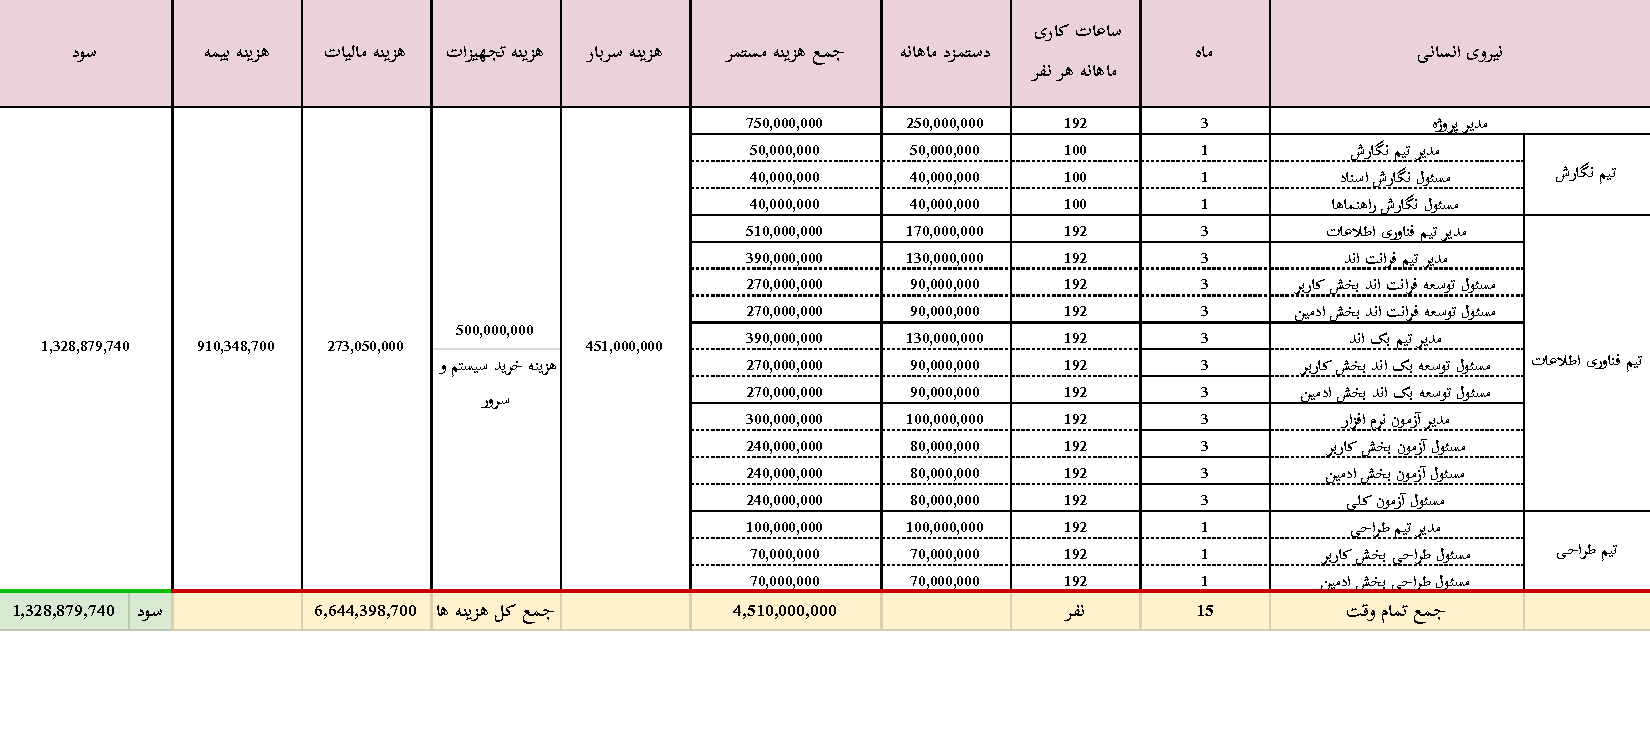
\includegraphics[width=\textwidth , scale=1.5]{appandecies/costs.pdf}}
  \end{figure}
  \captionof{table}[Short caption]{جدول هزینه‌های پروژه}
\end{center}

در محاسبه مقادیر هزینه موارد زیر باید مورد نظر قرار گرفته شوند:
\begin{itemize}
	\item{
	هزینه ها به ریال نوشته شده اند.	
	}
	\item{
	هزینه بیمه معادل با 16.67 درصد هزینه منابع انسانی برآورد شده است.	
	}
	\item{
	هزینه بیمه معادل با 16.67 درصد هزینه منابع انسانی برآورد شده است.	
	}
	\item {
	هزینه سربار معادل با 10 درصد هزینه منابع انسانی برآورد شده است.	
	}
	\item{
	هزینه مالیات معادل با 5 درصد هزینه منابع انسانی برآورد شده است.	
	}
	\item{
	مقدار سود معادل با 20 درصد هزینه کل برآورد شده است.	
	}
\end{itemize}